\chapter[Diagramas]{Diagramas}
Durante o desenvolvimento do projeto, alguns diagramas foram elaborados para sincronização de pensamento da equipe e entendimento coletivo.

Dentre os diagramas construídos, dois consistem no banco de dados, para entendimento da conexão entre as classes (Figura 5 e 6), enquanto sete consistem na aplicação (Figura 7, 8, 9, 10, 11, 12 e 13), para entendimento de suas mecânicas, da interação do usuário com o sistema, e do funcionamento interno. Os diagramas utilizados para a aplicação foram o casos de uso e diagrama de atividades.

Os diagramas elaborados foram:

 \subsection{Banco de Dados}

  \begin{figure}[!htb]
        \centering
        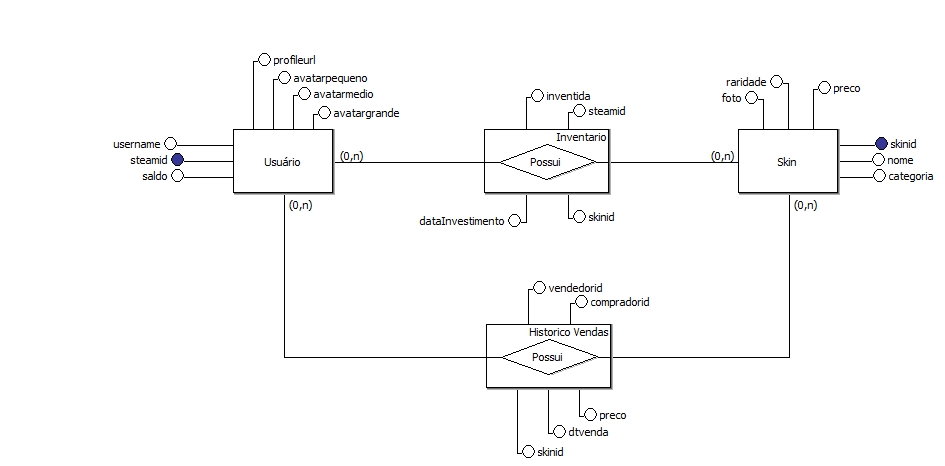
\includegraphics[scale=0.5]{Imagens/Relacionamento.png}
        \caption{Banco de Dados - Diagrama Entidade Relacionamento}
 \end{figure}

  \begin{figure}[!htb]
        \centering
        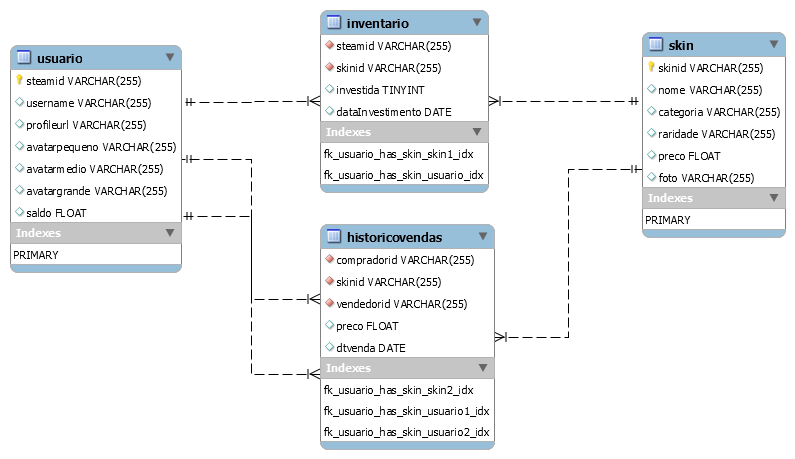
\includegraphics[scale=0.6]{Imagens/Logico.png}
        \caption{Banco de Dados - Modelo Lógico}
 \end{figure}

  \begin{figure}[!htb]
 \subsection{Casos de uso}
        \centering
        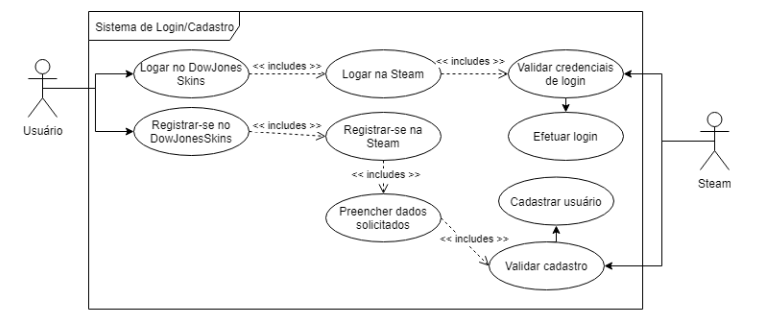
\includegraphics[scale=0.6]{Imagens/login.png}
        \caption{Caso de Uso - Login do usuário}
 \end{figure}

  \begin{figure}[!htb]
        \centering
        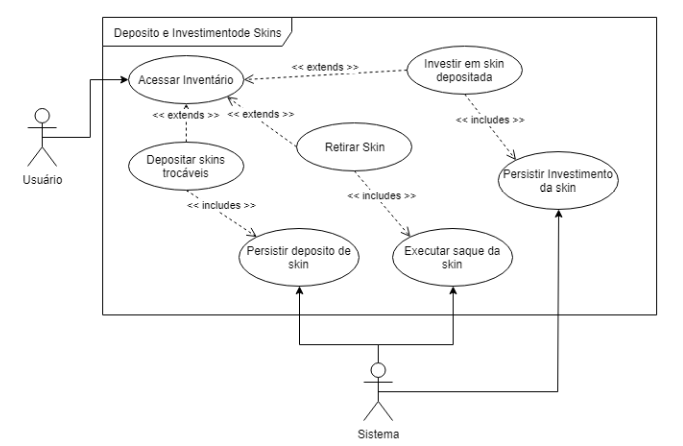
\includegraphics[scale=0.6]{Imagens/deposito.png}
        \caption{Caso de Uso - Depósito de Skins}
 \end{figure}

  \begin{figure}[!htb]
        \centering
        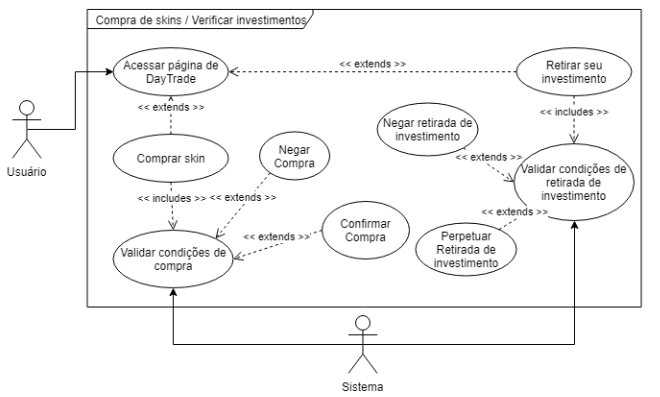
\includegraphics[scale=0.6]{Imagens/compra.png}
        \caption{Caso de Uso - Compra de Skins}
 \end{figure}

  \begin{figure}[!htb]
        \centering
        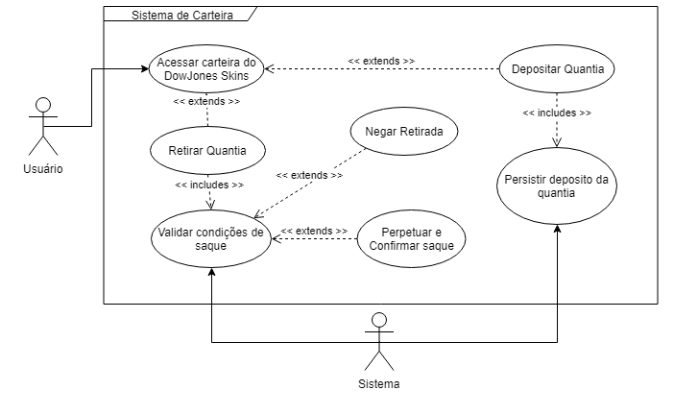
\includegraphics[scale=0.6]{Imagens/carteira.png}
        \caption{Caso de Uso - Carteira do usuário}
 \end{figure}

	\begin{figure}[!htb]
		\subsection{Diagramas de Atividade}
		\centering
		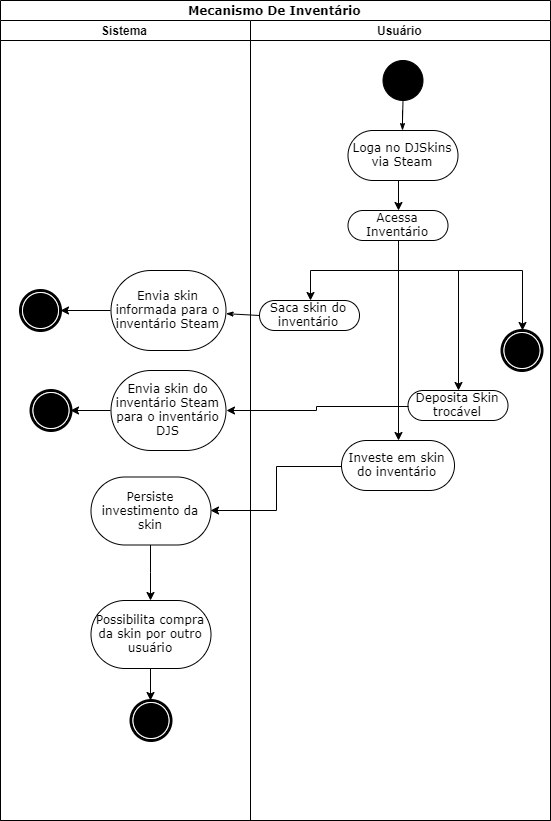
\includegraphics[scale=0.6]{Imagens/mec-inventario.png}
		\caption{Diagrama de Atividades - Mecanismo de Inventário}
	\end{figure}

	\begin{figure}[!htb]
		\centering
		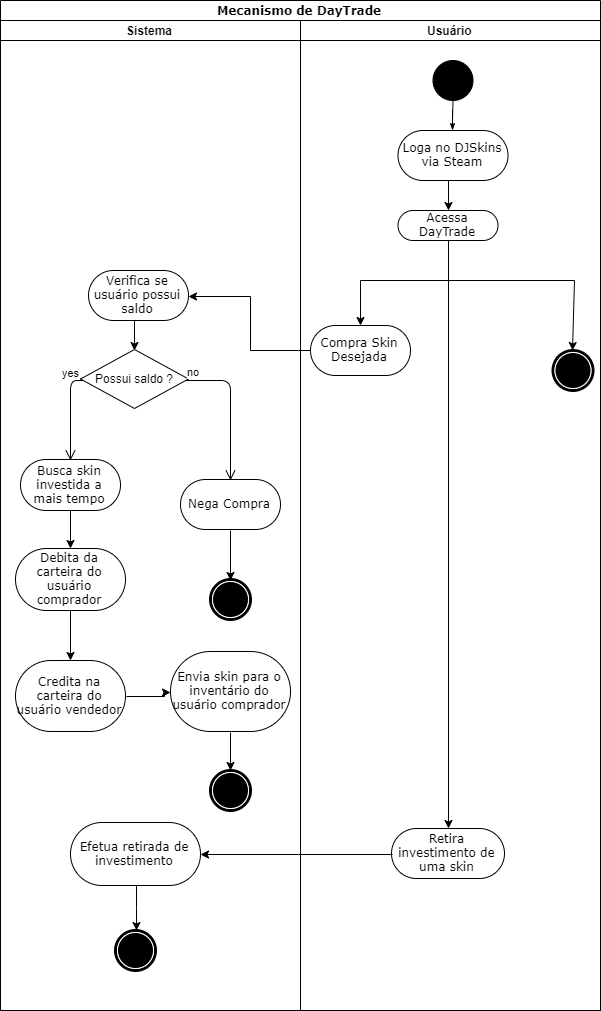
\includegraphics[scale=0.6]{Imagens/mec-daytrade.png}
		\caption{Diagrama de Atividades - Mecanismo de Day Trade}
	\end{figure}

	\begin{figure}[!htb]
		\centering
		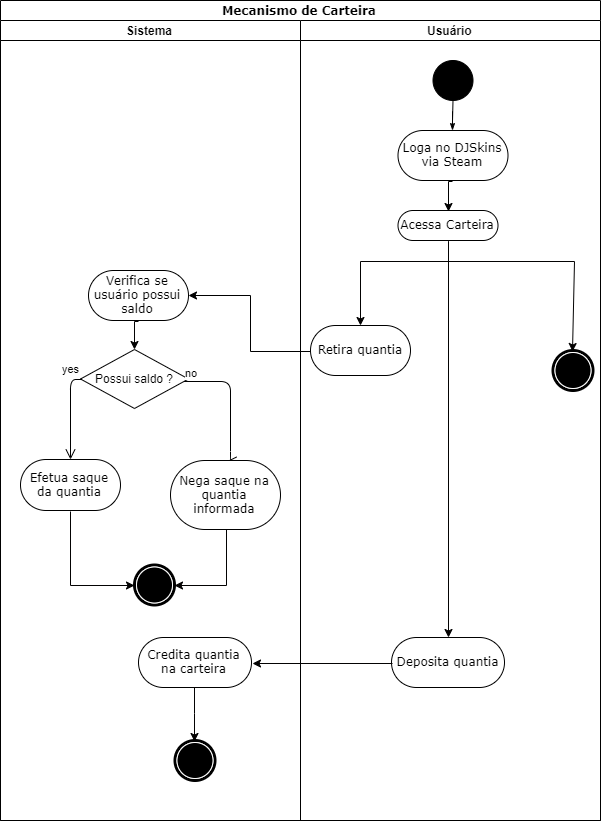
\includegraphics[scale=0.6]{Imagens/mec-carteira.png}
		\caption{Diagrama de Atividades - Mecanismo de Carteira}
	\end{figure}